\chapter{Annexe I}

\section{Matériels}

En ce que concerne les aspects matériels, le robot bimoteur Wifibot v2, qui transporte un ordinateur embarqué, sera utilisé comme plateforme mobile. L'acquisition des données est faite par une camera RGB-D portée par une tourelle qui permet son orientation indépendamment du positionnement du robot. Par rapport au choix logiciel, l'environnement robotique ROS a été adopté pout avoir les bibliothèques pour gérer les nuages de points, Freenect, OpenNi2 et PCL - Point Cloud Library, et d'autres nombreux outils de contrôle du robot et sauvegarde d'informations.

\subsection{ Plateforme mobile } 
\noindent
\begin{tabular}{cc}
 \begin{minipage}{0.5\textwidth} 
 \textbf{Robot Wifibot v2} \\ \textbf{Dimensions:}\\Hauteur : 18 cm \\ Largeur : 35 cm \\ Longueur : 30 cm \\ Distance entre roues : 0.32 cm \\ Diamètre des roues : 0.18 cm   \end{minipage}
 & 
 \begin{minipage}{0.5\textwidth}
	\begin{figure}[H]
	  \subfloat{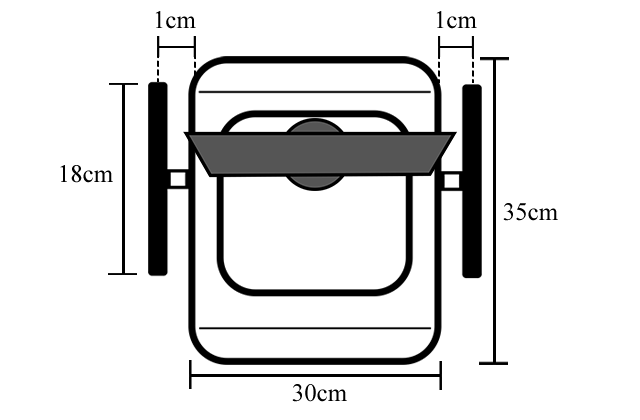
\includegraphics[width=\textwidth]{wbot_mesures.png}}
	\end{figure}
  \end{minipage}
\end{tabular}

\noindent
\begin{tabular}{cc}
\begin{minipage}{0.5\textwidth}  \textbf{Oridnateur portable embarqué :} \\ HD : 8 Go \\ RAM : 2 Go \\ Batterie : 12V NiMH 3.8A 9000mAH \\ Processeur : Intel\textsuperscript{\textregistered} Atom\textsuperscript{TM} N270 @ 1.60GHz \\ Systèm opérationnel : Ubuntu 14.04 \\ Version ROS : ROS Indigo \end{minipage} 
 & 
 \begin{minipage}{0.5\textwidth}
	\begin{figure}[H]
	  \subfloat{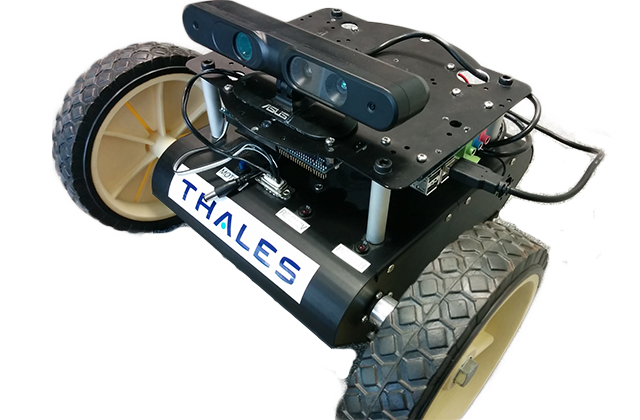
\includegraphics[width=\textwidth]{real_wbot.png}}
	\end{figure}
  \end{minipage}
\end{tabular}

\subsection{Description Ordinateur Portable}
\noindent
\begin{tabular}{cc}
\begin{minipage}{0.5\textwidth}
\textbf{HP Pavilion g6} \\
Processeur :  Intel\textsuperscript{\textregistered} Core\textsuperscript{TM} i5-3230M @ 2.60GHz \\
HD : 750Go \\
RAM : 4Go \\

Systèm opérationnel : Ubuntu 14.04 \\
Version ROS : ROS Indigo \\
\end{minipage}
	 & 
	\begin{minipage}{0.5\textwidth}
		\begin{figure}[H]
		  \subfloat{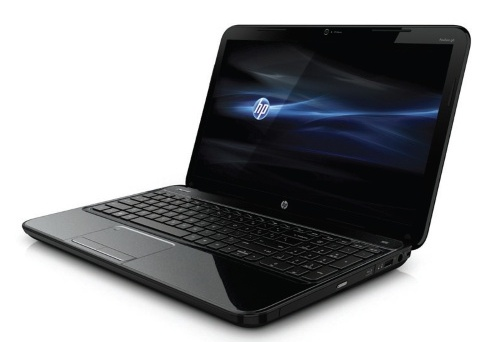
\includegraphics[width=\textwidth]{hp.jpg}}
		\end{figure}
	\end{minipage}
\end{tabular}

% {
%   \raggedleft
%   \begin{tikzpicture} 
%     \node (asus) {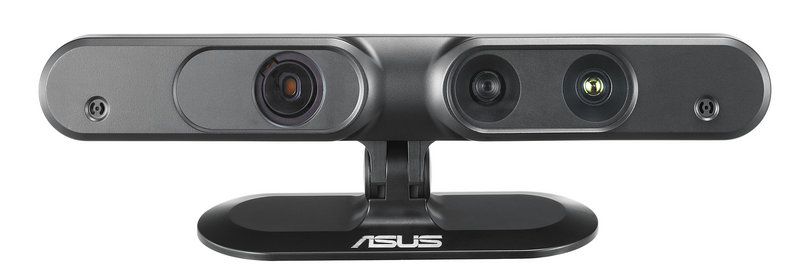
\includegraphics[width=0.4\textwidth]{xtion.jpg}};
%     \node [left=0.5cm of asus.north west, yshift=-5mm]{sdfsf};
%   \end{tikzpicture}
% }

\subsection{Capteur RGB-D}
\noindent
\begin{tabular}{cc}
	\begin{minipage}{0.5\textwidth} \textbf{Asus Xtion PRO LIVE} \\
	\textbf{Distance d'utilisation : }\\
	de 0.8 à 3.5 mètres \\
	\textbf{Range de vision : } \\
	58\degree Horizontal, 45\degree Vertical, 70\degree Diagonal \\
	\textbf{Resolution : } \\
	VGA (640x480) : 30 fps \\
	\textbf{Utilisation intérieur}
	\end{minipage}
	 & 
	\begin{minipage}{0.5\textwidth}
		\begin{figure}[H]
		  \subfloat{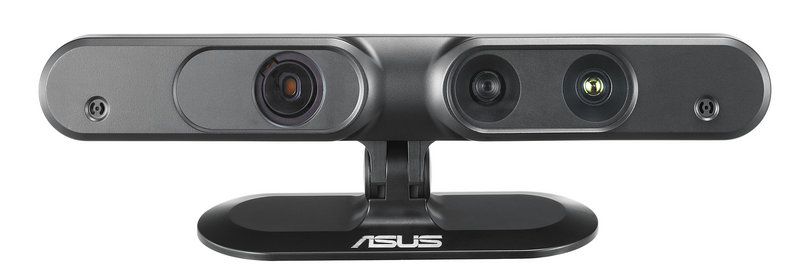
\includegraphics[width=\textwidth]{xtion.jpg}}
		\end{figure}
	\end{minipage}
\end{tabular}



\section{Base de données }

\begin{figure}[H]
  \subfloat{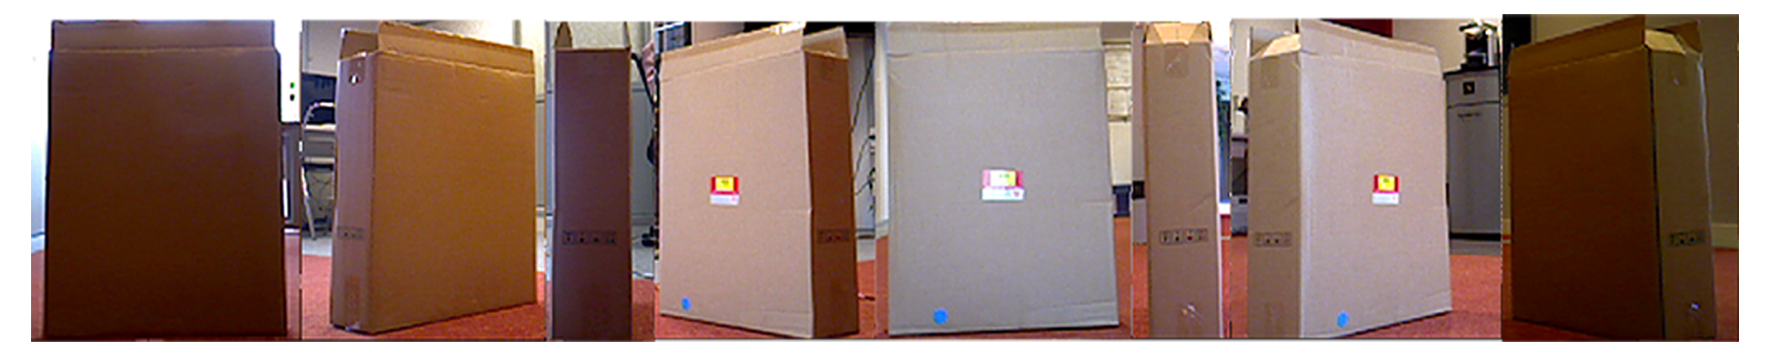
\includegraphics[width=\textwidth]{box_seq.png}}
\end{figure}

\begin{figure}[H]
  \subfloat{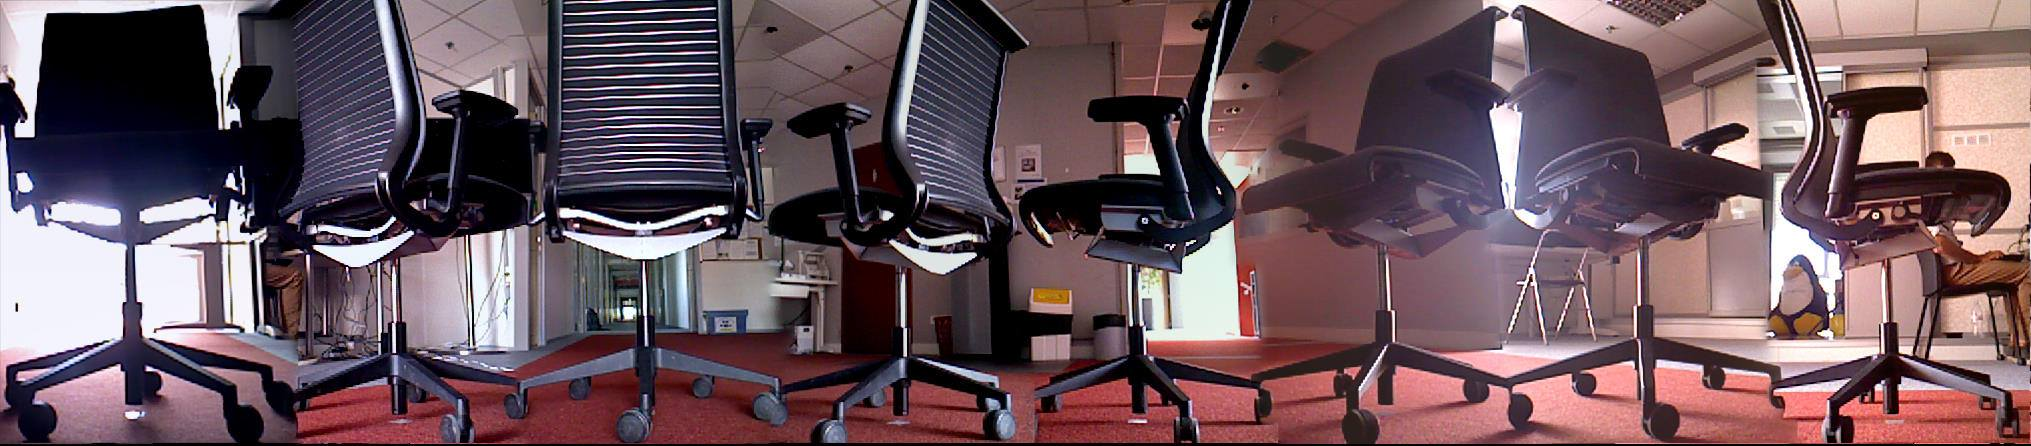
\includegraphics[width=\textwidth]{chair_db.jpg}}
\end{figure}

\begin{figure}[H]
  \subfloat{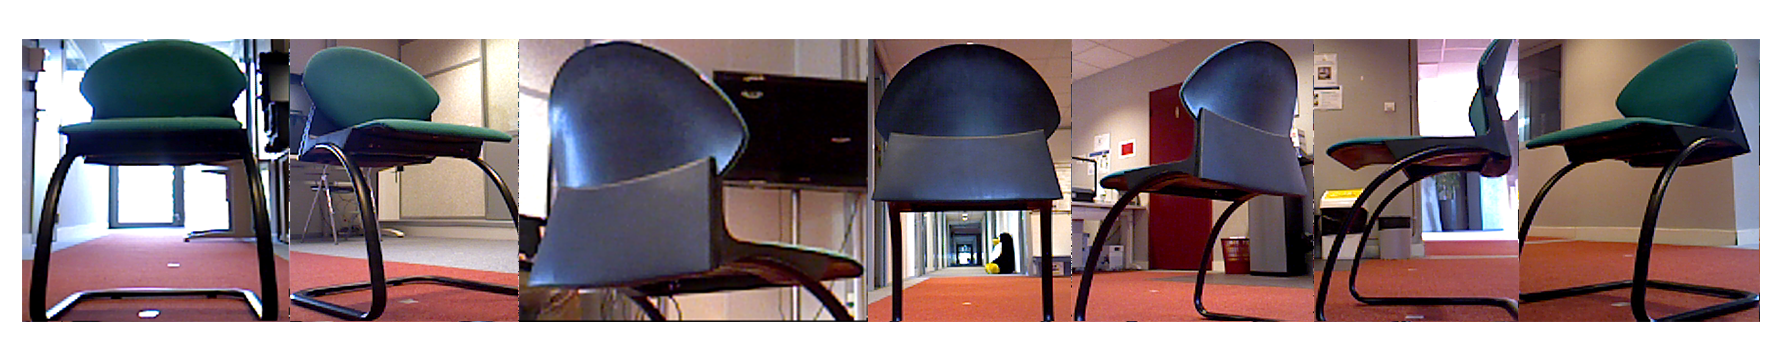
\includegraphics[width=\textwidth]{chair_seq.png}}
\end{figure}

\begin{figure}[H]
  \subfloat{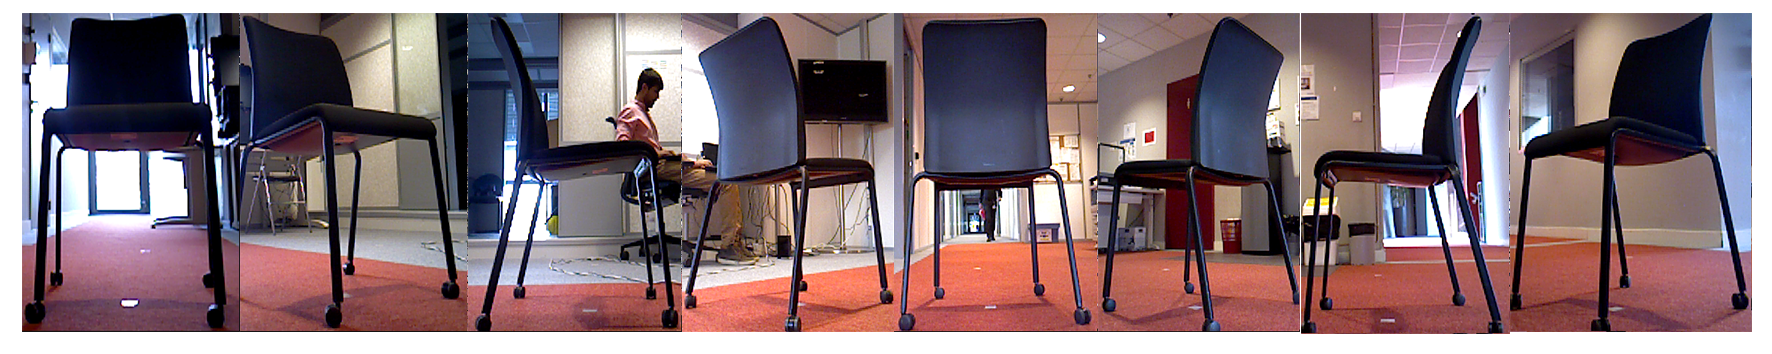
\includegraphics[width=\textwidth]{chair4w.png}}			
\end{figure}


\subsection{Restrictions logiciels}
L' ordinateur embarqué a un puissance de calcul reduit ce que ne permet pas que le node d'acquisition \(openni2\_launch\) tourne correctment. La solution pour l'instant c'était de connecter le capteur Asus sur l'ordinateur portable HP.

\section{ Segmentation }

\subsection{ Paramètres }

\begin{itemize}
\item Distance maximale au capteur : 3 m
\item Distance pour qu'un point soit considéré comme appartenant au plan : 5 cm
\item Taille du \textit{grid} de voxalization : 2 cm
\item Rayon d'estimation de la normale : 2 cm
\item Aire de \textit{smoothing} de la normale : 10 $cm^2$
\item Distance minimal du plan du sol pour qu'il soit considére comme partie de l'objet : 3 cm
\end{itemize}

La plus parts de valeurs étaient choisis telle comme ils était proposé dans la librarie PCL. Quelque autre ont été modifiés pour atteint charactéristique attendue.

\subsection { Floor Detection } 

The major concern goal of the algorithm is to well estimate the floor plan coordinates. From that, other plans like walls could be inferred, supposing they have a fixed geometrical relation. The RANSAC algorithm provide a reasonable solution to the problem and it is already implemented in the PCL library.

Some parameters need to be set, such as deviation from the plan mathematical model.

The parameters used for the robot are described at the annex section.


\subsection{Estimation de la normale}

Pour constituer les informations géométriques l'estimation de la normale du point est d'extrême importance. 

Sont calcul est fait de la manière suivant :
1. Un nombre de voisins est choisi 
2. Ces point *servem* à trouver des paramètres de l'équation du plan tangent et, par consequent, la normale correspondent.

Le méthode adopté pour la bibliothéque PCL correspond à prendre un certain nombre de plus proches voisins définis par un seiul. Un petit seil rendre le calcul faux et un grand prend en compte points distants que peuvent ne pas faire partie du plan estimé.

\url{http://www.pointclouds.org/documentation/tutorials/vfh_recognition.php#vfh-recognition} \\

\url{http://pointclouds.org/documentation/tutorials/fpfh_estimation.php} \\

\url{https://github.com/PointCloudLibrary/pcl/wiki/Overview-and-Comparison-of-Features} \\

\subsection { RANSAC } 

The RANSAC algorithm is a learning method to estimate a given model parameters. Contrary to other estimation algorithms, which considers the whole data represenetative to model estimation, RANSAC suppose the existance of \textbf{inliers or consensus} and \textbf{outliers}  and uses a voting scheme to select between reliable data, that must follow two assumptions: 

\begin{itemize}
\item Noisy data will not vote consistenly for a single model - (few outliners) 
\item Enough good features voting for the same model - (few missing data)
\end{itemize}

\subsubsection{The RANSAC algorithm}

The iterative algorithm is composed of two different stages : 
\begin {itemize}
\item Sample minimal data from dataset requerid to first estimate model parameters.
\item Given a threshold error, it selects data points that are consistent to the model created in the first step.
\end {itemize}

\begin{itemize}
\item Random hypoythetical inliers subset
\item Find model parameters
\item All data tested according to a loss function that determine the \textit{consensus}
\item Finishes when a sufficient number of point belongs to the \textit{consensus}
\end{itemize}

{ \large{\color{blue} If the variables are linear and normally distributed the Bayes filter becomes equal to the Kalman filter.}}

%% \caption{My algorithm}\label{euclid}
%% \begin{algorithmic}[1]
%%   \Procedure{RANSAC}{}
%%   \State $\textit{stringlen} \gets \text{length of }\textit{string}$
%%   \State $i \gets \textit{patlen}$
%%   \BState \emph{top}:
%%   \If {$i > \textit{stringlen}$} \Return false
%%   \EndIf
%%   \State $j \gets \textit{patlen}$
%%   \BState \emph{loop}:
%%   \If {$\textit{string}(i) = \textit{path}(j)$}
%%   \State $j \gets j-1$.
%%   \State $i \gets i-1$.
%%   \State \textbf{goto} \emph{loop}.
%%   \State \textbf{close};
%%   \EndIf
%%   \State $i \gets i+\max(\textit{delta}_1(\textit{string}(i)),\textit{delta}_2(j))$.
%%   \State \textbf{goto} \emph{top}.
%%   \EndProcedure
%% \end{algorithmic}
%% \end{algorithm}

\section {Descripteurs}
\subsection{Point Feature Histogram - PFH}

Le PFH incorporé les notions de courbure des objets par le calcul de
l'écart entre les normales de points. Ce descripteur peut être calculé
localement ou globalement, en changeant l'importance du rayon de
comparaison. Il est la base d'une grande famille de descripteurs, desquels
quelques-uns seront expliqués dans la suite.

En revenant à son calcul, l'histogramme est évalué à partir des pairs
de points à l'intérieur d’un ensemble prédéfini. D'abord, un repère
initial, illustré dans l'image *9* est établis sachant le vecteur distance normalisé et les deux
normales. Ensuite, trois angles, qui correspondent à la transformation
angulaire entre les deux normales, et la distance euclidienne entre le
deux points sont estimés. Ces quatres valeurs seront considérés comme
features pour réduire l’espace initial de douze dimensions - coordonnées
et normales des dois point - à un espace de quatre dimension.


\begin{equation*}
  {\mathsf u} = \boldsymbol{n}_s \qquad
  {\mathsf v} =  {\mathsf u} \times \frac{(\boldsymbol{p}_t-\boldsymbol{p}_s)}{{\|\boldsymbol{p}_t-\boldsymbol{p}_s\|}_{2}}  \qquad
  {\mathsf w} = {\mathsf u} \times {\mathsf v}
\end{equation*}

\begin{figure}[H]
  \centering
  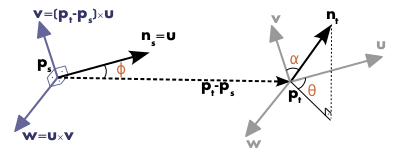
\includegraphics[width=0.6\textwidth]{pfh_frame.png}
  % \caption{{\color{blue} Image d'explication du repère}.}
\end{figure}


Puis, les normales sont traduites en features angulaires décrit par les équations :
\begin{equation*}
  \alpha = {\mathsf v} \cdot \boldsymbol{n}_t  \qquad
  \phi   = {\mathsf u} \cdot \frac{(\boldsymbol{p}_t - \boldsymbol{p}_s)}{d} \qquad
  \theta = \arctan ({\mathsf w} \cdot \boldsymbol{n}_t, {\mathsf u} \cdot \boldsymbol{n}_t) \qquad
  d={\|\boldsymbol{p}_t-\boldsymbol{p}_s\|}_2 
\end{equation*}

La prochaine étape c'est de calculer l'histogramme en-soi. Un
subdivision du range de valeur de chaque feature angulaire, 
normalisés pour rester dans le même intervalle trigonométrique,
est faite et chaque cellule du histogramme est incrémenté dès
qu'une feature tombe dans cet intervalle. 

Le PFH se présente robuste à des différents échelles de densité de points et de bruit, au même temps que invariant à les transformations affines. Des inconvénients vient de la dépendance de la qualité de l'estimation de la normale\footnote{ Une discussion des méthodes présentés sur PCL est mis dans les annexes.}.

\subsection{Fast Point Feature Histogram - FPFH}

L'avènement du FPFH viens de la motivation de réduire la complexité de
calcule du descripteur PFH, $ O(nk^2) $, pour un nuage avec $n$ points 
où chaqu'un des points à $k$ voisins . Pour cela, l'algorithme au
lieu de calculer la relation bidirectionnelle entre tous deux points 
de l’ensemble définis, les features de chaque point sont pondérées 
par les voisins à l'intérieur d'un rayon de recherche, selon la formule
au-dessous :

$$FPFH(\boldsymbol{p}_q) = SPFH(\boldsymbol{p}_q) + {1 \over k}
\sum_{i=1}^k {{1 \over \omega_k} \cdot SPFH(\boldsymbol{p}_k)}$$

Cette procédure résulte dans une complexité O(n*k). Le gain en vitesse est considérable,
ce qui permet des applications en temps réelles. De plus, pour éviter une perte d'information considérable, le FPFH
incorpore quelques point externes au rayon de voisinage, mais que sont compris dans un rayon de taille.

\subsection{Viewpoint Feature Histogram- VFH}

Le VFH, différemment du rapport entre PFH et FPFH, c'est une extension
du deuxième descripteur où la variance de point de vue est prise en
compte. De forme succincte, des angles entre la normale de chaque point
et la direction principale d'observation est concaténée à l’histogramme
provenant du SPFH (Simplified PFH). En gardant le repère utilisé dans
les descripteurs d'avant, le vecteur direction principale est défini
par la différence entre l'origine du capteur jusqu'au centroide du
\textit{cluster}. Ce résultat permet, au même temps, de reconnaitre
l'objet et son orientation spatiale, et, par conséquent, c'est le
feature utilisé dans les premières expériences.

\subsection{Clustered Viewpoint Feature Histogram - CVFH} CVFH -
Clustered VFH - est une feature semi-global capable de gérer
occlusions partiels, mauvaise segmentation et bruit par la
décomposition du \textit{cluster}, segmenté comme objet, en sous-clusters de
structure spatiale homogène. Le descripteur est obtenu d'après un premier
filtrage de zones de haute gradient de courbure, considérés comme zones de
transitions entre surfaces, et, puis, et l'estimation de l'histogramme VFH pour chaque surface 
donnée par l'algorithme \textit{point growing}. Ainsi, pour un seul objet, le CVFH ne
généré pas un seul histogramme VFH, mais un vecteur des histogrammes.
En revanche, le découpement exige un soin un plus avec la résolution des surfaces pour
quelles restent représentatives de l'objet.

\begin{figure}[H]
  \subfloat[PFH ]{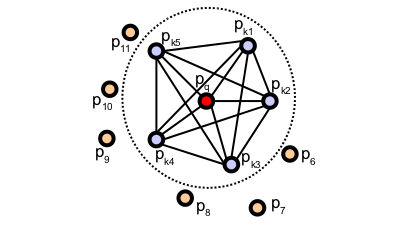
\includegraphics[width=4.5cm]{pfh_diagram.png}}
  \subfloat[FPFH]{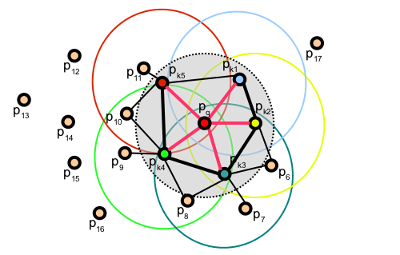
\includegraphics[width=4.5cm]{fpfh_diagram.png}}
  \subfloat[subcaption]{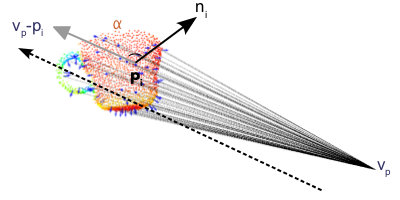
\includegraphics[width=6cm]{second_component.jpg}}		
\end{figure}


\textit{L'Universidad de León } a fait un compte rendu des
\textit{features} implementés sur PCL dans le lien *[8]*. Plus
d'information sur les descripteur et ses implementations sur la
librarie PCL peuvent être retrouvés sur le site
internet \url{http://pointclouds.org}.

Les images sont sauvegardées à l'aide de la librarie OpenCv dans le format 8\_U et .png (Portable Network Graphics).

Les nauges de points sont sauvegardées dans le format .pcd (Point Cloud Data).

Pour sauvegarder les information *provenientes* de la segmentation, les [it]topics de sorti sont souscrit avec rosbag pendent le deplacement du robot. Les messages sauvegardes sont le suivants :

\begin{itemize}
\item v\_objects\_clouds : Vector de nuages de points obtenues pour chaque objet 

\item v\_objects\_image\_and\_mask : Sousimages et mask de chaque objet

\item v\_object\_

\end{itemize}

\subsection{Fusion de données}

L'estimation de l’odométrie diverge au long du temps dû à
l'accumulation d'erreurs mesure. Cette divergence est encore plus
considérable . Dans l'autre côté, l'utilisation du senseur RGB-D
estime la distance au centroïde de chaque objet. Une correspondance
entre les objets de deux observations consécutives nous donné une
autre repère de positionnement. Un couplage des deux mesure, une
provenant de l’encodeur moteur et l'autre du capteur infrarouge, fait
que l'odométrie doive être

\section{Planning de Travail}
\begin{itemize}
\item[\checkmark] Mise en place de l'architecture et des protocoles de communication entre composants physiques.
\item[\checkmark] Étude bibliographique initiale pour situer le travail par rapport à l'existant.
\item[\checkmark] Implémentation de l'asservissement d'une caméra PTZ par rapport au retour d'un algorithme de tracking.
\item[\checkmark] Aperçu de certaines limitations de la caméra PTZ qui a été remplacée par une caméra RGB-D.
\item[\checkmark] Utilisation d'un algorithme de segmentation d'objets possibles dans la scène.
\item[\checkmark] Asservissement en boucle ouvert du robot pour la création de la base de données.
\item[\checkmark] Premiers tests pour l'acquisition de la base des données.
\item Résolution des problèmes trouvés lors des premiers tests pour la création de la base de données.
\item Validation de la base de données. Représentativité et reproduction.
\item Étude approfondie de l’état de l'art des modèles et méthodes qui puissent être utiles pour notre problème.
\item Mise en place de la solution et du modèle proposé.
\item Premiers tests et ajustements nécessaires.
\item Mise en œuvre de la solution complète.
\item Validation finale.    
\end{itemize}
